\section{Diskussion}
\label{sec:Diskussion}

Die Ergebnisse zur Untersuchung der Grenzfrequenzen mittels Durchlasskurve und Theorie lauten
\begin{align*}
  \nu_{1} &= \input{g1.tex}, \\
  \nu_{1, \text{theorie}} &= \input{g1_t.tex}, \\
  \nu_{2} &= \input{g2.tex}, \\
  \nu_{2, \text{theorie}} &= \input{g2_t.tex}.
\end{align*}
Es zeigt sich eine relative Abweichung des Messwerte zu den Theoriewerten von
\begin{align*}
  \increment\nu_{1} &= 1,3\:\%, \\
  \increment\nu_{2} &= 0,9\:\%,
\end{align*}
wobei die relative Abweichung nach
\begin{equation}
f = \frac{\lvert N - x \rvert }{N}
\label{eqn:rel_err}
\end{equation}
mit einem Theoriewert $N$ sowie einem Messwert $x$ berechnet werden.\\

Die Schwankungen der aufgenommenen Durchlasskurve, dargestellt in Abbildung \ref{fig:durchlass}, lassen sich dadurch erklären, dass der Wellenwiderstand frequenzabhängig ist.
Dies wird jedoch bei dieser Messung vernachlässigt.
Es entstehen daher Teilreflexionen, welche sich vor allem bei den Schwankungen jener Frequenzen äußern, die weit von der Frequenz entfernt sind, nach der der Wellenwiderstand ursprünglich ausgerichtet wurde.
Dennoch lassen sich die Grenzfrequenzen gut erkennen.\\
Die Abbildung \ref{fig:dispersion_fertig} spiegelt die beiden Äste der Dispersionsrelation wieder.
Prolematisch war es, dass der Frequenzgenerator für höhere Frequenzen eine grobere Messskala verwendet, und die Einstellung ebendieser Frequenzen sich als schwierig gestaltet hat.
Trotz dieser Schwierigkeiten beim Justieren der gewünschten Lissajous-Figuren, was sich letztendlich im Fehlen eines Wertes bemerkbar macht, liegen die gemessenen Werte auf den berechneten Theorieästen.
Größere Abweichungen im höheren Frequenzbereich lassen sich durch den oben genannten Fehler vollständig erklären.\\
\begin{figure}[H]
  \centering
  \includegraphics[height=8cm]{blödmann.jpg}
  \caption{Im Experiment genutzter Frequenzgenerator: Es fällt auf, dass die Messskala im hohen Frequenzbereich ungenau wird.}
  \label{fig:bloedmann}
\end{figure}
Bei der Bestimmung der Eigenfrequenzen und dem in Abbildung \ref{fig:phasengeschwindigkeiten} dargestellten Diagramm ergeben sich große Abweichungen.
Ein systematischer Fehler bei dieser Messung liegt im benutzten Frequenzgenerator, welcher die Frequenz konstant abfallen lässt.
%Aus welchem Grund auch immer ._________. kP
Bei näherer Betrachtung der hier bestimmten Eigenfrequenzen ist aufgefallen, dass diese eine starke systematische Ähnlichkeit zu den Frequenzen aufweisen, welche bei der Betrachtung der Dispersionsrelation in Kapitel \ref{sec:dis} bestimmt wurden.
Diese Frequenzen, welche in Tabelle \ref{tab:dispersion} dargestellt sind, weichen lediglich alle nach oben ab.
Diese Ähnlichkeit lässt sich dadurch erklären, dass bei der Aufgabenstellung in Kapitel \ref{sec:dis} Frequenzen gesucht wurden, bei denen sich eine Phasenverschiebung von $\pi$ zwischen dem ersten und letztem Kondensator ergibt.
Ebendiese Bedingung ist jedoch auch für die Eigenfrequenzen erfüllt.
Tragen wir also die Frequenzen aus Tabelle \ref{tab:dispersion} mit den dazugehörigen Phasengeschwindigkeiten in das Diagramm in Abbildung \ref{fig:phasengeschwindigkeiten} ein, so ergibt sich das in Abbildung \ref{fig:neucool} dargestelle Bild.
\begin{figure}[H]
  \centering
  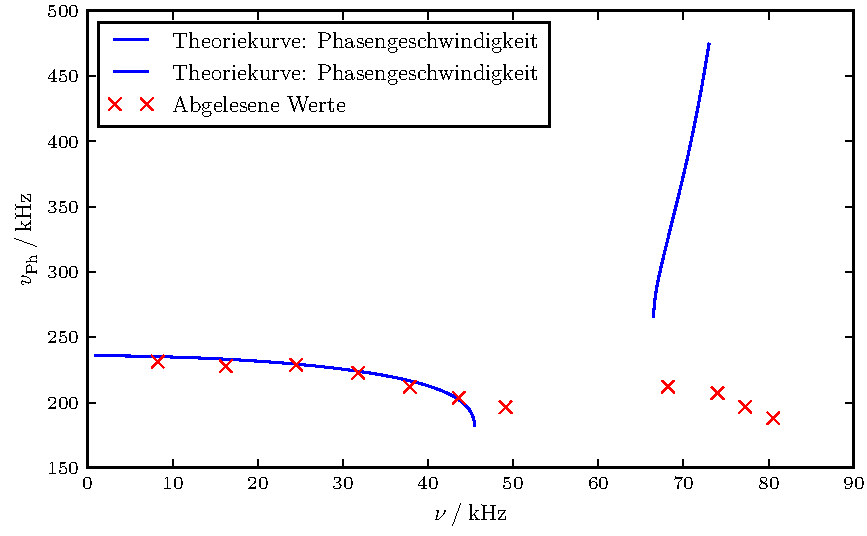
\includegraphics{neu.pdf}
  \caption{Phasengeschwindigkeiten der in Abschnitt \ref{sec:dis} bestimmten Frequenzen der LC-Kette sowie dazugehörige Theoriewerte.}
  \label{fig:neucool}
\end{figure}
Es fällt auf, dass die hier angegebenen Werte deutlich besser mit der Theorie zusammenpassen.
Die weiterhin vorhandenen Abweichungen bei hoheren Frequenzen lassen sich ebenfalls durch die Schwierigkeiten des Frequenzgenerators bei hohen Frequenzen erklären.\\
Im Allgemeinen kann der Grund für diese Abweichung daran liegen, dass das Ablesen der Lissajous-Figuren schneller durchgeführt werden konnte als das Ablesen der Spannungsmaxima.
Dementsprechend sind die Frequenzen dort zu stark abgefallen und die Messwerte verfälscht worden.


%Zur a:
%Die Kurve sieht so komisch aus, weil der Wellenwiderstand frequenzabhängig ist aber ja nicht geändert wird. Also haben wir Reflexionen.
%Die Werte sehen aber echt geil aus.
%
%Zur b:
%Höhere Frequenzen waren Kacke abzulesen. Deswegen sind die Werte nicht so genau.
%Sehen aber trotzdem geil aus.
%
%Zur c:
%
%
%Zur d:
%Spannung nimmt nach hinten ab: Wegen ohmschen Verlusten? (Macht das Sinn, weil wegen Wechselspannung?)
%
%Nicht 0 am Spannungsbauch weil wegen Reflexion weil wegen frequenzabhängigen Wellenwiderstand
